\documentclass[twoside,utf8]{article}
\usepackage{lipsum} % Package to generate dummy text throughout this template
\usepackage{comment}
\usepackage{amsmath, amssymb}
\usepackage{eulervm}
%\usepackage{mathpazo}
%\usepackage[math]{anttor}
%\usepackage{cmbright}
%\usepackage{mathastext}
\usepackage{amsthm}
\usepackage[lined,boxed,commentsnumbered]{algorithm2e}
\usepackage[usenames,dvipsnames]{xcolor}
\usepackage{graphicx}
\usepackage[T1]{fontenc} % Use 8-bit encoding that has 256 glyphs
\linespread{1.05} % Line spacing - Palatino needs more space between lines
\usepackage{microtype} % Slightly tweak font spacing for aesthetics
\usepackage[hmarginratio=1:1,top=32mm,columnsep=20pt]{geometry} % Document margins
\usepackage{multicol} % Used for the two-column layout of the document
\usepackage[hang, small,labelfont=bf,up,textfont=it,up]{caption} % Custom captions under/above floats in tables or figures
\usepackage{booktabs} % Horizontal rules in tables
\usepackage{float} % Required for tables and figures in the multi-column environment - they need to be placed in specific locations with the [H] (e.g. \begin{table}[H])
\usepackage[colorlinks=false,hyperfootnotes=false]{hyperref} % For hyperlinks in the PDF
\usepackage{lettrine} % The lettrine is the first enlarged letter at the beginning of the text
\usepackage{paralist} % Used for the compactitem environment which makes bullet points with less space between them
\usepackage{abstract} % Allows abstract customization
\usepackage{titlesec} % Allows customization of titles
\usepackage{caption}
\usepackage{subcaption}
\usepackage{tikz}
\usetikzlibrary{calc}

\renewcommand{\abstractnamefont}{\normalfont\bfseries} % Set the "Abstract" text to bold
\renewcommand{\abstracttextfont}{\normalfont\small\itshape} % Set the abstract itself to small italic text
\renewcommand\thesection{\Roman{section}} % Roman numerals for the sections
\renewcommand\thesubsection{\Roman{subsection}} % Roman numerals for subsections
\titleformat{\section}[block]{\large\scshape\centering\bfseries}{\thesection.}{1em}{} % Change the look of the section titles
\titleformat{\subsection}[block]{\scshape\bfseries}{\thesubsection.}{1em}{} % Change the look of the section titles

\newcommand{\EQU}[1] { \begin{equation*} \begin{split} #1 \end{split} \end{equation*} }
\newcommand{\EQUn}[1] { \begin{equation} \begin{split} #1 \end{split} \end{equation} }
\newcommand{\PAR}[2]{ \frac{\partial #1}{\partial #2}}
\newcommand{\ket}[1] { |#1\rangle }
\newcommand{\expe}[1]{ \langle #1 \rangle }
\newcommand{\bra}[1] { \langle #1 | }
\newcommand{\braket}[2] { \langle #1 | #2 \rangle }
\newcommand{\NOTE}[1]{ {\color{red}#1}}

%----------------------------------------------------------------------------------------
%	Theorems and definitions
%----------------------------------------------------------------------------------------

\theoremstyle{plain}
\newtheorem{theorem}{Theorem}
\newtheorem{proposition}{Proposition}
\newtheorem{lemma}{Lemma}
\newtheorem*{corollary}{Corollary}
\newtheorem*{remark}{Remark}

\theoremstyle{definition}
\newtheorem{definition}{Definition}
\newtheorem{conjecture}{Conjecture}
\newtheorem*{example}{Example}
\theoremstyle{remark}
\newtheorem*{note}{Note}
\newtheorem{case}{Case}

%----------------------------------------------------------------------------------------
%	TITLE SECTION
%----------------------------------------------------------------------------------------

\title{\vspace{-15mm}\fontsize{24pt}{10pt}\selectfont\textbf{Classification of complex semisimple Lie algebras using Dynkin diagrams}} % Article title

\author{
\large
\textsc{August Geelmuyden} %\thanks{A thank you or further information}
\\[2mm] % Your name
\normalsize University of Oslo \\ % Your institution
%\normalsize \href{mailto:john@smith.com}{john@smith.com} % Your email address
\vspace{-5mm}
}
\date{}

%----------------------------------------------------------------------------------------

\begin{document}

\maketitle % Insert title

%\tableofcontents*

%----------------------------------------------------------------------------------------
%	INTRODUCTION
%----------------------------------------------------------------------------------------
\section{Introduction}
The most developed theory of continuous symmetries of mathematical objects is the theory of Lie groups. The local structure of a Lie group, it turns out, is completely determined by a structure called a Lie algebra, which is related to the tangent space of the Lie group at the identity element. This text is concerned with root systems and their relation to Dynkin diagrams. The properties of a certain type of Lie algebras, know as the complex, semisimple Lie algebras, can be captured in a root system. The classification of root systems therefore give a classification of Lie groups. 

While the first section explores the connection between roots systems and the so called Cartan matrix, the succeeding section studies root systems and Dynkin diagrams. Here the reduced, irreducible root systems are classification into the four families $A_n$, $B_n$, $C_n$ and $D_n$, together with the five exceptions $G_2$, $F_4$, $E_6$, $E_7$ and $E_8$. In the end, a brief look at the definitions and results, without proof, needed to understand the connection between root systems and Lie algebras is presented. 

This text is written as a part of the course MAT2000 at the University of Oslo collaborating with \textit{Niels Bonten}. The proofs and structure of the text rests heavily on the two books \textit{Serres, J.P, Complex semisimple Lie algebras}\cite{Serre} and \textit{Erdmann, K. and Wildon, Introduction to Lie algebras}\cite{LieAlgebrasIntroduction}. 





\begin{comment}
Lie groups common. Classified by Dynkin diagrams. The link is the concept of root systems. We will study root systems. Then the cartan matrix and coxeter graphs. These are clasified. Coxeter graphs is not sufficient -- needs Dynkin diagrams to properly represent all reduced, irreducible root systems. In the end we take a brief look at the factorization of semisimple complex Lie algebras and the relation to root systems.
\begin{itemize}
\item Results
\item What is about to happen in each section
\item Do not state importance of theorem
\item State assumptions: Any vectorspace is implicitly thought of as finite dimensional
\end{itemize}
\end{comment}

%----------------------------------------------------------------------------------------
%	ROOT SYSTEMS
%----------------------------------------------------------------------------------------
\section{Root systems}

In the following sections, all vector spaces are assumed to be finite dimensional over the field $\mathbb{R}$.

\subsection{Symmetry of a vector}

\begin{definition}
Let $\alpha\neq 0$ be a vector in a vector space $V$. Define the \textit{symmetry with the vector $\alpha$} as a linear transformation $s_\alpha \in Aut(V)$ satisfying
\begin{description}
\item[(S1)] $s_\alpha(\alpha)=-\alpha$.
\item[(S2)] $s_\alpha$ fixes a hyperplane $H$.
\end{description}
\end{definition}

\begin{proposition}
There exist at most one $s_\alpha$.
\end{proposition}
\begin{proof}
Let $\alpha\in V$ be a non-zero vector and let $s$ and $s'$ be two symmetries for $\alpha$. Since $\alpha$ extends the basis for $H$ to a basis for $V$ every vector $x\in V$ can be written in the form $x = \beta + C\alpha$ where $\beta \in H$ and $C$ is a constant from the underlying field. Then $s(x)=s(\beta)+Cs(\alpha) = \beta - C \alpha$ since $s$ is a symmetry for the vector $\alpha$. Similarly $s'$ is a symmetry for $\alpha$ so $s'(x)=\beta - C \alpha$ and thus $s'(x)=s(x)$. Since $x$ was arbitrarily chosen, the proof is complete.
\end{proof}

\noindent
If $V$ is a vector space then for every nonzero $\alpha \in V$ we may always construct a linear function $\alpha^* : V \rightarrow \mathbb{R}$ that vanishes on a hyperplane $H$ in $V$ and takes the value $2$ on $\alpha$. Since this imposes constraints on every basis element of $V$, the function $\alpha^*$ is uniquely determined by $\alpha$. Recalling that the dual space $V^*$ of $V$ consists of all linear functions from $V$ to $\mathbb{R}$ makes us able to rephrase the result; for each nonzero $\alpha \in V$ there exist a unique element $\alpha^*\in V^*$ which vanishes on a hyperplane $H$ and takes the value $2$ on $\alpha$.

\begin{proposition}
Every symmetry $s_\alpha$ is of the form $s_\alpha(x)=x-\alpha^*(x) \alpha$.
\end{proposition}
\begin{proof}
Since there exists at most one $s_\alpha$, it suffices to show that $s_\alpha(x)=x-\alpha^*(x ) \alpha$ is a symmetry for $\alpha$. First note that the map $x\mapsto \alpha^*(x) \alpha$ is a linear map by definition. Since $\alpha^*(\beta) = 0$ for all $\beta \in H$ it follows that $s_\alpha$ fixes $H$. Finally, since $\alpha^*(\alpha) = 2$, we have $s_\alpha(\alpha)=-\alpha$. 
\end{proof}

\noindent
Note that one immediate consequence is the existence of a unique symmetry $s_\alpha(x)=x-\alpha^*(x) \alpha$ for every nonzero vector $\alpha \in V$. 



\subsection{Root systems}
\begin{definition}
A subset $R\subseteq V$ is a \textit{root system} if
\begin{description}
\item[(R1)] $R$ does not contain $0$, is finite and spans $V$. 
\item[(R2)] For all $\alpha \in R$ there is a symmetry $s_\alpha$ with $s_\alpha(\beta)\in R$ for all $\beta \in R$.
\item[(R3)] For all $\alpha,\beta \in R$ there is some $n\in \mathbb{Z}$ so that $s_\alpha(\beta)-\beta = n\alpha$.
\end{description}
\end{definition}

\noindent
Notice that (R3) is equivalent to saying that $\alpha^*$, the unique element in $V^*$ that vanishes on a hyperplane $H$ and takes the value $2$ on $\alpha$, takes integer values on all $\beta \in R$. That is, $\alpha^*(\beta) \in \mathbb{Z}$ for all $\beta \in R$.

\begin{definition}
A root system $R$ is said to be \textit{reduced} if for all $\alpha \in R$ the only distinct vector in $R$ being proportional to $\alpha$ is $-\alpha$.
\end{definition}

\noindent
It follows that all reduced, one-dimensional root systems is of the form $R=\{\pm \alpha \}$ for some nonzero vector $\alpha \in V$. 

\begin{figure}[H]
\centering
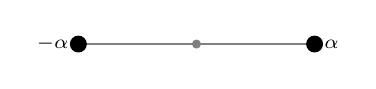
\begin{tikzpicture}[scale=1]
\def\cLine{gray}
\def\cDot{black}
\def\cText{black}
\def\u{1.5}
\def\r{0.1}
\coordinate (O) at (0,0);
\filldraw[\cLine] (O) circle[radius=0.05];
\draw[\cLine, thick] (O) -- (\u,0);
\filldraw[\cDot] (\u,0) circle[radius=\r] node[\cText,anchor=west]{\scriptsize$\alpha$};
\draw[\cLine, thick] (O) -- (-\u,0);
\filldraw[\cDot] (-\u,0) circle[radius=\r] node[\cText,anchor=east]{\scriptsize$-\alpha$};
%\draw[\cLine, thick] (O) -- (0,\u);
%\filldraw[\cDot] (0,\u) circle[radius=\r] node[\cText,anchor=south]{\scriptsize$\beta$};
%\draw[\cLine, thick] (O) -- (0,-\u);
%\filldraw[\cDot] (0,-\u) circle[radius=\r] node[\cText,anchor=north]{\scriptsize$-\beta$};
\end{tikzpicture}
%\caption{The only one-dimensional, reduced root system.}
%\label{fig:OneDimRootSystem}
\end{figure}





\subsection{Weyl group}

\begin{definition}[Weyl group]
If $R$ is a root system let the \textit{Weyl group}, denoted $W$, be the subgroup of $\mbox{Aut}(V)$ generated by all symmetries $s_\alpha$ with vectors from $R$. 
\end{definition}

\noindent 
Now we may think of (R2) as the criterion that the Weyl group leaves the root system invariant, $WR=R$.

\begin{proposition} \label{prop:symBilinForm}
There exists a symmetric, positive definite bilinear form $(\cdot,\cdot):V\times V \rightarrow \mathbb{F}$ that is invariant under the Weyl group.
\end{proposition}
\begin{proof}
If $A$ is a symmetric, positive definite matrix then $B(x,y)=x^TAy$ is a symmetric, positive definite bilinear form on $V$.
Let $B(\cdot,\cdot)$ be such a bilinear form on $V$ and consider the form $(\cdot,\cdot)$ defined by
\[
(x,y) = \sum_{w\in W} B(wx,wy).
\]
Clearly $(\cdot,\cdot)$ is both symmetric and bilinear. Further, since $B(\cdot,\cdot)$ is positive definite $(x,x)=0$ means that $B(wx,wx)=0$ for all $w\in W$. Since $B(\cdot,\cdot)$ is positive definite then $wx=0$ for all $w\in W$. Hence $x=0$, meaning that $(\cdot,\cdot)$ is positive definite. It remains only to show that $(\cdot,\cdot)$ is invariant under $W$. If $t\in W$ then
\[
(tx,ty) = \sum_{w\in W} B(wtx,wty) = \sum_{w\in Wt} B(wx,wy) = \sum_{w\in W} B(wx,wy),
\]
so $(\cdot,\cdot)$ is indeed invariant under $W$.
\end{proof}

\noindent
Unless otherwise stated, $(\cdot,\cdot)$ will hereby refer to the bilinear form in the above proposition. Now, observing that
\[
s_\alpha(x)=x-2\frac{(\alpha,x)}{(\alpha,\alpha)}\alpha
\]
is a symmetry for $\alpha$ we may, remembering that every symmetry is of the form $x-\alpha^*(x)\alpha$, identify 
\[
\alpha^*(x)=2\frac{(\alpha,x)}{(\alpha,\alpha)}.
\]
Hence we may reformulate (R3) by demanding that $2\frac{(\alpha,x)}{(\alpha,\alpha)} \in \mathbb{Z}$ for all $x\in R$. To simplify notation we let
\[
n(\alpha,\beta) = 2\frac{(\alpha,\beta)}{(\alpha,\alpha)}
\]
allowing us to write any symmetry with a vector $\alpha$ in the form
\[
s_\alpha(\beta)=\beta-n(\alpha,\beta)\alpha.
\]

\begin{definition}
The \textit{length} of an element $\alpha \in R$ is defined as $|\alpha|=\sqrt{(\alpha,\alpha)}$. The \textit{angle} $\theta$ between two elements $\alpha$ and $\beta$ of a root system $R$ is given by the relation $(\alpha,\beta)=|\alpha| |\beta| \cos \theta$.
\end{definition}

\noindent
Observing that if $R$ is a root system and $\alpha,\beta \in R$ then
\[
n(\alpha,\beta) = 2\frac{|\beta|}{|\alpha|} \cos \theta
\mbox{ and }
n(\alpha,\beta)n(\beta,\alpha)=4\cos^2 \theta
\]
leads us to conclude that the only integer values $n(\alpha,\beta)n(\beta,\alpha)$ can take are $0,1,2,3,4$. If $\alpha$ and $\beta$ are non-proportional then there are only the seven possibilities listen in table \ref*{tab:RootsAndAngles}.

\begin{table}[H]
\caption{Possible values for $n(\alpha,\beta)$ with corresponding angles and relative lengths.}
\label{tab:RootsAndAngles}
\begin{center}
\begin{tabular}{r r r r}
%\toprule
$n(\alpha,\beta)$ 	& $n(\beta,\alpha)$ & $\theta$ 		&	$\frac{|\alpha|^2}{|\beta|^2}$			\\ \hline 
$0$ 				& $0$ 				& $\pi/2$ 		&	 -- 		\\ 
$1$ 				& $1$ 				& $\pi/3$ 		&	$1$  		\\ 
$-1$ 				& $-1$ 				& $2\pi/3$ 		&	$1$			\\ 
$1$ 				& $2$ 				& $\pi/4$ 		&	$2$	\\ 
$-1$ 				& $-2$ 				& $3\pi/4$ 		&	$2$	\\ 
$1$ 				& $3$ 				& $\pi/6$ 		&	$3$	\\ 
$-1$ 				& $-3$ 				& $5\pi/6$ 		&	$3$	\\ 
%\bottomrule
\end{tabular}
\end{center}
\end{table}


\begin{proposition} \label{prop:AlphaBetaDiffInR}
If $\alpha$ and $\beta$ are elements in a root system $R$ with $(\alpha,\beta)>0$, then $\alpha-\beta \in R$.
\end{proposition}
\begin{proof}
If $(\alpha,\beta)>0$ then $n(\alpha,\beta)>0$ and according to table \ref*{tab:RootsAndAngles} we have either $n(\alpha,\beta)=1$ or $n(\beta,\alpha)=1$. If $n(\beta,\alpha)=1$ then $\alpha-\beta = \alpha-n(\beta,\alpha)\beta =  s_\beta(\alpha) \in R$. Similarly, if $n(\alpha,\beta)=1$ then $\alpha-\beta = -\beta+n(\alpha,\beta)\alpha=-s_{\alpha}(\beta)\in R$. That is, in both cases $\alpha-\beta \in R$.
\end{proof}

\noindent
Now, observe that
\[
\begin{aligned}
|s_\beta(\alpha)|^2 
&= \left(\alpha-n(\alpha,\beta)\beta,\alpha-n(\alpha,\beta)\beta\right) \\
&= |\alpha|^2-2n(\alpha,\beta)|\alpha||\beta|\cos \phi+n(\alpha,\beta)^2|\beta|^2 = |\alpha|^2.
\end{aligned}
\]
This means that $(\alpha,s_\beta(-\alpha))=|\alpha|^2 \cos \theta$ where $\theta$ is the angle subtended by $\alpha$ and $s_\beta(-\alpha)$. Interestingly, if $\phi$ is the angle subtended by $\alpha$ and $\beta$ then
\[
\begin{aligned}
|\alpha|^2 \cos \theta 
&= (\alpha,s_\beta(-\alpha))
= -(\alpha,\alpha)+2\frac{(\alpha,\beta)^2}{(\beta,\beta)} \\
&= |\alpha|^2 \left( 2\cos^2 \phi - 1 \right)
= |\alpha|^2 \cos 2\phi.
\end{aligned}
\]
Hence if there are two roots that subtend an angle $\phi$, then there exists a pair of roots subtending an angle $2\phi$. In fact, this implies the existence of roots subtending an angle of any integer multiple of $\phi$.
 With this in mind, we can use table \ref*{tab:RootsAndAngles} to find the possible two dimensional reduced root systems.



\begin{figure}[h]
\begin{subfigure}[b]{0.5\textwidth} % A1 * A1 =============================================================================
\centering
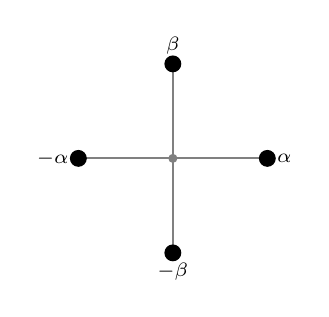
\begin{tikzpicture}[scale=1]
\def\cLine{gray}
\def\cDot{black}
\def\cText{black}
\def\u{1.2}
\def\r{0.1}
\coordinate (O) at (0,0);
\filldraw[\cLine] (O) circle[radius=0.05];
\draw[\cLine, thick] (O) -- (\u,0);
\filldraw[\cDot] (\u,0) circle[radius=\r] node[\cText,anchor=west]{\scriptsize$\alpha$};
\draw[\cLine, thick] (O) -- (-\u,0);
\filldraw[\cDot] (-\u,0) circle[radius=\r] node[\cText,anchor=east]{\scriptsize$-\alpha$};
\draw[\cLine, thick] (O) -- (0,\u);
\filldraw[\cDot] (0,\u) circle[radius=\r] node[\cText,anchor=south]{\scriptsize$\beta$};
\draw[\cLine, thick] (O) -- (0,-\u);
\filldraw[\cDot] (0,-\u) circle[radius=\r] node[\cText,anchor=north]{\scriptsize$-\beta$};
\end{tikzpicture}
\caption*{$(A_1\times A_1)$} \label{fig:A1A1}
\end{subfigure}
\begin{subfigure}[b]{0.5\textwidth} % A2 =============================================================================
\centering
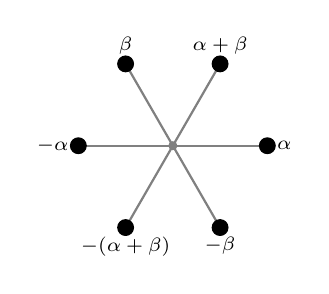
\begin{tikzpicture}
\def\cLine{gray}
\def\cDot{black}
\def\cText{black}
\def\u{1.2}
\def\r{0.1}
\def\t{60}
\coordinate (O) at (0,0);
\filldraw[\cLine] (O) circle[radius=0.05];
\draw[\cLine, thick] (O) -- (\u,0);
\filldraw[\cDot] (\u,0) circle[radius=\r] node[\cText,anchor=west]{\scriptsize$\alpha$};
\draw[\cLine, thick] (O) -- (-\u,0);
\filldraw[\cDot] (-\u,0) circle[radius=\r] node[\cText,anchor=east]{\scriptsize$-\alpha$};
\draw[\cLine, thick] (O) -- ({\u*cos(\t)},{\u*sin(\t)});
\filldraw[\cDot] ({\u*cos(\t)},{\u*sin(\t)}) circle[radius=\r] node[\cText,anchor=south]{\scriptsize$\alpha+\beta$};
\draw[\cLine, thick] (O) -- (-{\u*cos(\t)},-{\u*sin(\t)});
\filldraw[\cDot] (-{\u*cos(\t)},-{\u*sin(\t)}) circle[radius=\r] node[\cText,anchor=north]{\scriptsize$-(\alpha+\beta)$};
\draw[\cLine, thick] (O) -- ({\u*cos(2*\t)},{\u*sin(2*\t)});
\filldraw[\cDot] ({\u*cos(2*\t)},{\u*sin(2*\t)}) circle[radius=\r] node[\cText,anchor=south]{\scriptsize$\beta$};
\draw[\cLine, thick] (O) -- (-{\u*cos(2*\t)},-{\u*sin(2*\t)});
\filldraw[\cDot] (-{\u*cos(2*\t)},-{\u*sin(2*\t)}) circle[radius=\r] node[\cText,anchor=north]{\scriptsize$-\beta$};
\end{tikzpicture}
\caption*{$(A_2)$} \label{fig:A2}
\end{subfigure}
\begin{subfigure}[b]{0.5\textwidth} % B2 =============================================================================
\centering
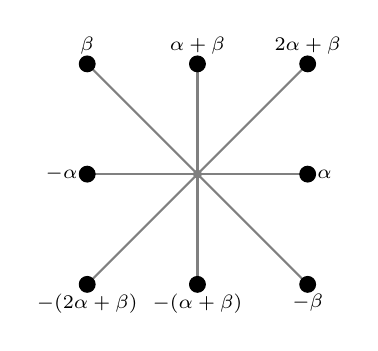
\begin{tikzpicture}
\def\cLine{gray}
\def\cDot{black}
\def\cText{black}
\def\u{1.4}
\def\r{0.1}
\def\t{45}
\coordinate (O) at (0,0);
\filldraw[\cLine] (O) circle[radius=0.05];
\draw[\cLine, thick] (O) -- (\u,0);
\filldraw[\cDot] (\u,0) circle[radius=\r] node[\cText,anchor=west]{\scriptsize$\alpha$};
\draw[\cLine, thick] (O) -- (-\u,0);
\filldraw[\cDot] (-\u,0) circle[radius=\r] node[\cText,anchor=east]{\scriptsize$-\alpha$};
\draw[\cLine, thick] (O) -- ({sqrt(2)*\u*cos(\t)},{sqrt(2)*\u*sin(\t)});
\filldraw[\cDot] ({sqrt(2)*\u*cos(\t)},{sqrt(2)*\u*sin(\t)}) circle[radius=\r] node[\cText,anchor=south]{\scriptsize$2\alpha+\beta$};
\draw[\cLine, thick] (O) -- (-{sqrt(2)*\u*cos(\t)},-{sqrt(2)*\u*sin(\t)});
\filldraw[\cDot] (-{sqrt(2)*\u*cos(\t)},-{sqrt(2)*\u*sin(\t)}) circle[radius=\r] node[\cText,anchor=north]{\scriptsize$-(2\alpha+\beta)$};
\draw[\cLine, thick] (O) -- ({\u*cos(2*\t)},{\u*sin(2*\t)});
\filldraw[\cDot] ({\u*cos(2*\t)},{\u*sin(2*\t)}) circle[radius=\r] node[\cText,anchor=south]{\scriptsize$\alpha+\beta$};
\draw[\cLine, thick] (O) -- (-{\u*cos(2*\t)},-{\u*sin(2*\t)});
\filldraw[\cDot] (-{\u*cos(2*\t)},-{\u*sin(2*\t)}) circle[radius=\r] node[\cText,anchor=north]{\scriptsize$-(\alpha+\beta)$};
\draw[\cLine, thick] (O) -- ({sqrt(2)*\u*cos(3*\t)},{sqrt(2)*\u*sin(3*\t)});
\filldraw[\cDot] ({sqrt(2)*\u*cos(3*\t)},{sqrt(2)*\u*sin(3*\t)}) circle[radius=\r] node[\cText,anchor=south]{\scriptsize$\beta$};
\draw[\cLine, thick] (O) -- (-{sqrt(2)*\u*cos(3*\t)},-{sqrt(2)*\u*sin(3*\t)});
\filldraw[\cDot] (-{sqrt(2)*\u*cos(3*\t)},-{sqrt(2)*\u*sin(3*\t)}) circle[radius=\r] node[\cText,anchor=north]{\scriptsize$-\beta$};
\end{tikzpicture}
\caption*{$(B_2)$} \label{fig:B2}
\end{subfigure}
\begin{subfigure}[b]{0.5\textwidth} % G2 =============================================================================
\centering
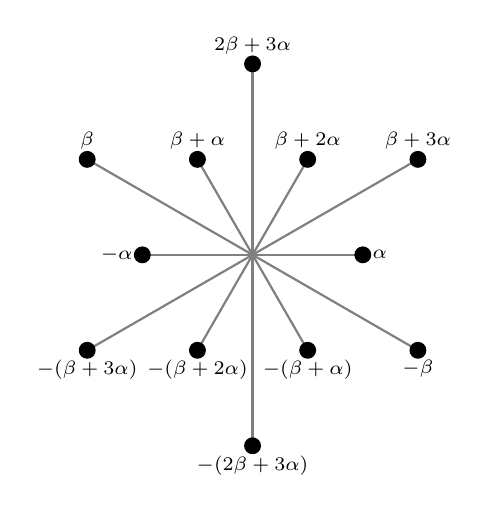
\begin{tikzpicture}
\def\cLine{gray}
\def\cDot{black}
\def\cText{black}
\def\u{1.4}
\def\r{0.1}
\def\t{30}
\coordinate (O) at (0,0);
\filldraw[\cLine] (O) circle[radius=0.05];
\draw[\cLine, thick] (O) -- (\u,0);
\filldraw[\cDot] (\u,0) circle[radius=\r] node[\cText,anchor=west]{\scriptsize$\alpha$};
\draw[\cLine, thick] (O) -- (-\u,0);
\filldraw[\cDot] (-\u,0) circle[radius=\r] node[\cText,anchor=east]{\scriptsize$-\alpha$};
\def\t{30}
\def\A{sqrt(3)}
\draw[\cLine, thick] (O) -- ({\A*\u*cos(\t)},{\A*\u*sin(\t)});
\draw[\cLine, thick] (O) -- ({-\A*\u*cos(\t)},{-\A*\u*sin(\t)});
\filldraw[\cDot] ({\A*\u*cos(\t)},{\A*\u*sin(\t)}) circle[radius=\r] node[\cText,anchor=south]{\scriptsize$\beta+3\alpha$};
\filldraw[\cDot] ({-\A*\u*cos(\t)},{-\A*\u*sin(\t)}) circle[radius=\r] node[\cText,anchor=north]{\scriptsize$-(\beta+3\alpha)$};
\def\t{60}
\def\A{1}
\draw[\cLine, thick] (O) -- ({\A*\u*cos(\t)},{\A*\u*sin(\t)});
\draw[\cLine, thick] (O) -- ({-\A*\u*cos(\t)},{-\A*\u*sin(\t)});
\filldraw[\cDot] ({\A*\u*cos(\t)},{\A*\u*sin(\t)}) circle[radius=\r] node[\cText,anchor=south]{\scriptsize$\beta+2\alpha$};
\filldraw[\cDot] ({-\A*\u*cos(\t)},{-\A*\u*sin(\t)}) circle[radius=\r] node[\cText,anchor=north]{\scriptsize$-(\beta+2\alpha)$};
\def\t{90}
\def\A{sqrt(3)}
\draw[\cLine, thick] (O) -- ({\A*\u*cos(\t)},{\A*\u*sin(\t)});
\draw[\cLine, thick] (O) -- ({-\A*\u*cos(\t)},{-\A*\u*sin(\t)});
\filldraw[\cDot] ({\A*\u*cos(\t)},{\A*\u*sin(\t)}) circle[radius=\r] node[\cText,anchor=south]{\scriptsize$2\beta+3\alpha$};
\filldraw[\cDot] ({-\A*\u*cos(\t)},{-\A*\u*sin(\t)}) circle[radius=\r] node[\cText,anchor=north]{\scriptsize$-(2\beta+3\alpha)$};
\def\t{120}
\def\A{1}
\draw[\cLine, thick] (O) -- ({\A*\u*cos(\t)},{\A*\u*sin(\t)});
\draw[\cLine, thick] (O) -- ({-\A*\u*cos(\t)},{-\A*\u*sin(\t)});
\filldraw[\cDot] ({\A*\u*cos(\t)},{\A*\u*sin(\t)}) circle[radius=\r] node[\cText,anchor=south]{\scriptsize$\beta+\alpha$};
\filldraw[\cDot] ({-\A*\u*cos(\t)},{-\A*\u*sin(\t)}) circle[radius=\r] node[\cText,anchor=north]{\scriptsize$-(\beta+\alpha)$};
\def\t{150}
\def\A{sqrt(3)}
\def\n{$\beta$}
\draw[\cLine, thick] (O) -- ({\A*\u*cos(\t)},{\A*\u*sin(\t)});
\draw[\cLine, thick] (O) -- ({-\A*\u*cos(\t)},{-\A*\u*sin(\t)});
\filldraw[\cDot] ({\A*\u*cos(\t)},{\A*\u*sin(\t)}) circle[radius=\r] node[\cText,anchor=south]{\scriptsize\n};
\filldraw[\cDot] ({-\A*\u*cos(\t)},{-\A*\u*sin(\t)}) circle[radius=\r] node[\cText,anchor=north]{\scriptsize$-$\n};
\end{tikzpicture}
\caption*{$(G_2)$} \label{fig:G2}
\end{subfigure}
\caption{
The four distinct two dimensional, reduced root systems.
}
\label{fig:PossibleRootSystemsInTwoDimensions}
\end{figure}



\subsection{Bases}
Looking at figure \ref*{fig:PossibleRootSystemsInTwoDimensions} we may observe that most of the information is superfluous. For example, in $A_2$ the existence and position of the roots $\alpha+\beta$ and $-(\alpha+\beta)$ follows directly from the criterions (R2) and (R3). This introduces the notion of a base for a root system.

\begin{definition}[base]
A set $B\subseteq R$ is called a \textit{base for the root system R} if it is a basis for $V$ and for all $\alpha \in R$ there is a set of integers $\{n_b\}$ with the same sign (all either $\geq 0$ or $\leq 0$) satisfying $\alpha = \sum_{b\in B} n_b b$. A root whose integer coefficients are non-negative is called a \textit{positive root} and a root whose integer coefficients are non-positive is called a \textit{negative root}.
\end{definition}

\begin{definition}[decomposability]
Let $R$ be a root system in a vector space $V$. For any $t\in V^*$ satisfying $t(\alpha)\neq 0$ for all $\alpha \in R$ define the set $R^+_t$ consisting of elements $\alpha \in R$ such that $t(\alpha)>0$. A root $\alpha \in R_t^+$ is said to be \textit{decomposable} if there exists $\beta,\gamma \in R^+_t$ so that $\alpha=\beta+\gamma$. A root that is not decomposable is said to be \textit{indecomposable}. We denote the set of all indecomposable roots in $R$ with respect to $t$ by $S_t$.
\end{definition}

\begin{lemma} \label{lem:leq0}
If $\alpha,\beta \in S_t$ then $(\alpha,\beta)\leq 0$.
\end{lemma}
\begin{proof}
Let $\alpha, \beta \in S_t$ and see that if $(\alpha,\beta)>0$, then proposition \ref*{prop:AlphaBetaDiffInR} gives that $\gamma=\alpha-\beta \in R$, where either $\gamma \in R^+_t$ or $-\gamma \in R^+_t$. In the first case $\alpha = \gamma+\beta$ is decomposable, and in the second case $\beta = \alpha+(-\gamma)$ is decomposable, both contradicting $\alpha,\beta \in S_t$.
\end{proof}

\begin{lemma} \label{lem:linIndep}
Let $t\in V^*$ and $A \subseteq V$ be such that $t(\alpha)>0$ for all $\alpha \in A$, and $(\alpha,\beta)\leq 0$ for all $\alpha,\beta \in A$. Then the vectors in $A$ are linearly independent.
\end{lemma}
\begin{proof}
It suffices to show that if $0=\sum_{\gamma\in A}m_\gamma \gamma$ then $m_\gamma=0$ for all $\gamma \in A$. Given such a linear combination we may always separate the negative terms from the positive terms writing it in the form
\[
\sum_{\gamma \in A_1} c_\gamma \gamma = \sum_{\gamma \in A_2}k_\gamma \gamma
\]
where $c_\gamma$ and $k_\gamma$ are non-negative coefficients and $A_1$ and $A_2$ are disjoint sets satisfying $A=A_1\cup A_2$. Now, if $v = \sum_{\gamma \in A_1}c_\gamma \gamma$ then 
\[
(v,v) =  \sum_{\gamma \in A_1} \sum_{\gamma' \in A_2} c_\gamma k_{\gamma'} (\gamma,\gamma') \leq 0
\]
since $(\alpha,\beta)\leq 0$ for all $\alpha,\beta \in A$. Since $(\cdot,\cdot)$ is positive definite, we must have $(v,v)=0$ and thus $v=0$. Now, since this means that $t(v)=t(0)=0$ we have
\[
t(v)=\sum_{\gamma \in A_1} c_\gamma t(\gamma)=0,
\]
but since $t(\gamma)>0$ for all $\gamma \in A_1$ we must have $c_\gamma=0$ for all $\gamma \in A_1$. An indentical argument shows that $k_\gamma=0$ for all $\gamma \in A_2$ which finalizes the proof.
\end{proof}

\begin{lemma} \label{lem:nonNegativeIntegers}
Each element of $R^+_t$ is a linear combination, with non-negative integer coefficients, of elements from $S_t$.
\end{lemma}
\begin{proof}
Let $I\subseteq R^+_t$ be set consisting of all elements $\alpha$ of $R^+_t$ not satisfying the statement. If $I$ is nonempty then we may choose the element $\alpha \in I$ with minimal $t(\alpha)$. Since $\alpha$ does not satisfy the above statement, it must be decomposable. Hence $\alpha=\beta+\gamma$ for $\beta,\gamma \in R^+_t$. But
\[
t(\alpha) = t(\beta)+t(\gamma)
\]
means that $\beta \notin I$ and $\gamma \notin I$ since $t(\beta)>0$ and $t(\gamma)>0$ and $t(\alpha)$ is minimal. But then $\alpha \notin I$, which contradicts the assumption that $I$ is nonempty.
\end{proof}

\begin{proposition}
For any $t\in V^*$ with $t(\alpha) \neq 0$ for all $\alpha \in R$, the set $S_t$ of all indecomposable roots is a base for $R$.
\end{proposition}
\begin{proof}
Since $R^+_t$ spans $V$, so must $S_t$. Moreover, the roots in $S_t$ are linearly independent according to lemma \ref*{lem:linIndep} and \ref*{lem:leq0}. 

Hence it remains only to show that for $\alpha \in R$ there is a set of integers $\{n_\beta\}$ with the same sign satisfying $\alpha = \sum_{\beta\in S_t} n_\beta \beta$. Now, if $\alpha \in R$ then either $\alpha \in R^+_t$ or $-\alpha \in R^+_t$. If $\alpha \in R^+_t$ then according to lemma \ref*{lem:nonNegativeIntegers} we can write 
\[
\alpha = \sum_{\gamma \in S_t} m_\gamma \gamma
\]
where $m_\gamma$ are non-negative integer coefficients. If $-\alpha \in R^+_t$ then 
\[
\alpha = \sum_{\gamma \in S_t} (-m_\gamma) \gamma.
\]
In both cases, $\alpha$ has been written as a linear combination, with integer coefficients of equal sign, of elements from $S_t$
\end{proof}


\begin{proposition} \label{prop:SisSt}
If $S$ is a base for $R$, then $S=S_t$ for some $t\in V^*$.
\end{proposition}
\begin{proof}
Let $t\in V^*$ with $t(\alpha)>0$ for all $\alpha \in S$ and let $R^+$ be the set of all positive roots. If $\alpha \in R^+_t$ then $t(\alpha)>0$. Since we may write $\alpha=\sum_{\gamma\in S}m_\gamma \gamma$ then 
\[
t(\alpha)=\sum_{\gamma\in S}m_\gamma t(\gamma)>0
\]
meaning that there is at least one $\gamma$ so that $m_\gamma>0$. Since $S$ is a base it follows that $m_\gamma \geq 0$ for all $\gamma \in S$. That is, $\alpha \in R^+$. Conversely, if $\alpha \in R^+$ then $\alpha=\sum_{\gamma\in S}m_\gamma \gamma$ with $m_\gamma \geq 0$ for all $\gamma\in S$ with at least one $\gamma$ satisfying $m_\gamma > 0$ . Then $t(\alpha)>0$ since $t(\gamma)>0$ for all $\gamma \in S$ by definition . Hence $R^+ = R^+_t$.

Now let $\alpha \in S_t \subseteq R^+_t = R^+$ and write 
\[
\alpha=\sum_{\gamma \in S} m_\gamma \gamma \mbox{ with } m_\gamma\geq 0 \mbox{ for all } \gamma \in S,
\]
which is possible since $S\subseteq R^+_t$ by definition of $t$. Since $\alpha$ is indecomposable and $S\subseteq R^+_t$ we must have $m_\gamma = 0$ for all but one $\gamma \in S$, which has a coefficient $m_\gamma=1$. Hence $\alpha = \gamma$ and therefore also $\alpha \in S$. This means that $S_t \subseteq S$. Since $S$ and $S_t$ are bases for the same vector space they must have the same number of elements, forcing us to conclude that $S=S_t$.
\end{proof}


\begin{lemma} \label{lemma:HalfTheSum}
Let $R$ be a reduced root system and $\alpha$ an element in its base $S$. If $R^+$ is the set of all the positive roots of $R$, then $R^+-\{\alpha\}$ is invariant under the symmetry $s_\alpha$. Moreover, if $\sigma$ is half the sum of all the roots in $R^+$ then $s_\alpha(\sigma)=\sigma-\alpha$ for all $\alpha \in S$.
\end{lemma}
\begin{proof}
If $\beta \in R^+-\{\alpha\}$ for some $\alpha\in S$, then 
\[
\beta = \sum_{\gamma\in S} m_\gamma  \gamma \mbox{ with } m_\gamma \geq 0 \mbox{ for all } \gamma \in S.
\]
Since $R$ is reduced there is no root in $R^+-\{\alpha\}$ that is proportional to $\alpha$. Hence there must exist $\gamma \in S$ with $\gamma \neq \alpha$ and $m_\gamma\neq 0$. Then, since $\alpha \in S$ the coefficient of $\gamma$ in $s_\alpha(\beta)=\beta-n(\beta,\alpha)\alpha$ is $m_\gamma$, which is positive. This linear combination is unique as it consists of basis elements only. Since $S$ is a base, $s_\alpha(\beta)$ has to be written as a linear combination of elements from $S$ with non-negative integer coefficients. That is, $s_\alpha(\beta)\in R^+-\{\alpha\}$. Since this holds for any $\beta \in R^+-\{\alpha\}$ we conclude that the set $R^+-\{\alpha\}$ is invariant under $s_\alpha$.

Now, if $\sigma_\alpha$ is half the sum of all the roots in $R^+-\{\alpha\}$ then $s_{\alpha}(\sigma_\alpha)=\sigma_\alpha$. Further, if $\sigma$ is half the sum of all roots from $R^+$ then $\sigma=\sigma_\alpha+\frac{1}{2}\alpha$ and thus $s_{\alpha}(\sigma)=\sigma_\alpha-\frac{1}{2}\alpha = \sigma - \alpha$.
\end{proof}

\begin{theorem} \label{thm:FourPoints}
If $W$ is the Weyl group of a reduced root system $R$ and $S$ is a base for $R$ then:
\begin{itemize}
\item[1)] For $t\in V^*$ there is $w\in W$ so that $(t \circ w^{-1})(\alpha)\geq 0$ for all $\alpha \in S$.
\item[2)] If $S'$ is a base for $R$, then there exists some $w \in W$ such that $w(S')=S$.
\item[3)] For all $\alpha \in R$ there exist $w \in W$ so that $w(\alpha)\in S$.
\item[4)] $W$ is generated by $s_\alpha$ for $\alpha \in S$.
\end{itemize}
\end{theorem}
\begin{proof}
We will first prove $1)$, $2)$ and $3)$ for the subgroup $W_S$ of $W$ generated by all the symmetries $s_\alpha$ for $\alpha \in S$ and later show that $W_S=W$.

Let $\sigma$ be half the sum of all the positive roots and choose $w\in W_S$ so that $t(w^{-1}\sigma)$ is maximal. It follows from lemma \ref*{lemma:HalfTheSum} that
\[
t(w^{-1}\sigma)\geq t(w^{-1}s_\alpha \sigma) = t(w^{-1} \sigma)-t(w^{-1} \alpha) \mbox{ for all } \alpha \in S.
\]
Hence $t(w^{-1} \alpha)\geq 0$ for all $\alpha \in S$.

For $2)$ note that if $t'\in V^*$ is chosen so that $t'(\alpha)>0$ for all $\alpha \in S'$ then it follows from $1)$ that there exists some $w\in W_S$ so that $t=t'\circ w^{-1}$ satisfies $t(\beta)\geq 0$ for all $\beta \in S$. Since any vector $\alpha \in R$ has coefficients of equal sign when written as a linear combination of elements from the base $S'$, and $t'(\alpha)>0$ for all $\alpha \in S'$, it follows that $t'(\alpha)\neq 0$ for all $\alpha \in R$.
Hence $t(\alpha) \neq 0$ for all $\alpha \in R$. According to proposition \ref*{prop:SisSt} we have $S=S_t$ and $S'=S_{t'}$ giving 
\[
S
=S_{t\circ w^{-1} \circ w}
=S_{t' \circ w}
=w(S_{t'})
=w(S').
\]

To prove $3)$ we must show that for $\alpha \in R$ there exists $w\in W_S$ so that $w(\alpha) \in S$. First define the hyperplane $L_\alpha = \{ t \in V^* | t(\alpha)=0 \}$ and see that since $R$ is reduced, the only other hyperplane that is not distinct from $L_\alpha$ is $L_{-\alpha}$. Hence it is possible to choose $t_0\in L_\alpha$ so that $t_0$ is not contained in any $L_\gamma$ for a root $\gamma$ different from $\pm \alpha$. This means that
\[
t_0(\alpha)=0 \mbox{ but } t_0(\gamma)\neq 0 \mbox{ for all } \gamma \in R-\{\pm \alpha\}.
\]
One can for some $\varepsilon>0$ strictly less than the minimal $|t_0(\gamma)|$ for $\gamma \in R-\{\pm \alpha\}$ find an element $t \in V^*$ so that $t(\alpha)=\varepsilon$. If $S_{t}$ is the base of $R$ corresponding to $t$ then we must have $\alpha\in S_{t}$, for if not then $\alpha = \beta + \gamma$ with $\beta,\gamma\in S_{t}$ which is contradicted by $t(\alpha)=t(\beta)+t(\gamma)>2\epsilon$. It follows from $2)$ that there is some $w\in W_S$ so that $w(S_t)=S$ and thus $w(\alpha) \in S$.

To prove that $W_S=W$ it suffices to show that if $\alpha \in R$ then $s_\alpha \in W_S$, since $W$ is generated by all symmetries of this form and $W_S\subseteq W$. If $\alpha \in R$ it follows from $3)$ that there exists $w\in W_S$ so that $w(\alpha)=\beta$ for $\beta \in S$. Since $n(w(\alpha),w(\beta))=n(\alpha,\beta)$ we have
\[
\begin{aligned}
s_\beta(x)
&= s_{w(\alpha)}(x)
= x-n(w(\alpha),x)w(\alpha)
= x-n(\alpha,w^{-1}(x))w(\alpha) \\
&= w\left( w^{-1}(x)-n(\alpha,w^{-1}(x))w^{-1}(\alpha) \right)
= (w \circ  s_\alpha \circ w^{-1})(x)
\end{aligned}
\]
meaning that $s_\alpha = w^{-1}\circ s_\beta \circ w$. Since this is a product of elements from $W_S$ it follows that $s_\alpha \in W_S$.
\end{proof}



\begin{corollary} \label{Cor:RisWS}
If $S$ is a base for a reduced root system $R$ with Weyl group $W$, then $R=WS$. 
\end{corollary}
\begin{proof}
From $3)$ in the previous theorem it follows that for any $\alpha \in R$ there is $w\in W$ so that $w(\alpha)=\beta$ with $\beta \in S$. Since $W$ is a group there exists an inverse $q\in W$ so that $(q \circ w)(x)=x$ implying that $\alpha = q(\beta)$. This gives $R \subseteq WS$, and since $R$ being a root system forces $WS \subseteq WR$ to be contained in $R$, we have no choice but to conclude that $R=WS$.
\end{proof}



\subsection{The Cartan matrix}

\begin{proposition}
Let $S$ and $S'$ be bases for the two root systems $R$ and $R'$ respectively, being subsets of the two vector spaces $V$ and $V'$. Let $\Phi: S \rightarrow S'$ be a bijection satisfying $n(\Phi(\alpha),\Phi(\beta))=n(\alpha,\beta)$ for all $\alpha,\beta \in S$. Then a unique isomorphism $f: V \rightarrow V'$ exists which is an extension of $\Phi$ to $R$.
\end{proposition}
\begin{proof}
First note that if $\alpha,\beta \in S$ then
\[
\left( s_{\Phi(\alpha)} \circ f \right)(\beta) 
= (s_{\Phi(\alpha)} \circ \Phi )(\beta)
= \Phi (\beta)-n\left({\Phi(\alpha)}, \Phi (\beta)\right){\Phi(\alpha)}
= \Phi (\beta)-n\left(\alpha,\beta\right){\Phi(\alpha)}
\]
and
\[
\left( f \circ s_{\alpha} \right) (\beta) 
= f\left(  \beta - n(\alpha, \beta )\alpha \right) 
= f(\beta) - n(\alpha, \beta )f(\alpha)
= \Phi(\beta) - n(\alpha, \beta )\Phi(\alpha).
\]
That is, $f \circ s_{\alpha} = s_{\Phi(\alpha)} \circ f $. If $W$ and $W'$ are the Weyl groups of $R$ and $R'$ respectively, then according to the corollary of theorem \ref*{thm:FourPoints} we have $R=WS$ and $R'=W'S'$ and according to the observation above $W'f=fW$. Thus $R' = W'S' = W'f(S) = f(WS) = f(R)$ meaning that $R$ is isomorphic to $R'$.
\end{proof}

\noindent
This illustrates that two root systems whose integers $n(\alpha,\beta)$ of base elements $\alpha$, $\beta$ coincide are isomorphic. That is to say, a root system $R$ is determined up to isomorphism by the set $\{n(\alpha,\beta)\}_{\alpha,\beta\in S}$ where $S$ is a base for $R$.

\begin{definition}[Cartan matrix]
Let $B=\{\alpha_i\}$ be a base for a root system $R$. The matrix with elements $C_{ij}=n(\alpha_i,\alpha_j)$ is called a \textit{Cartan matrix} for the root system $R$ with respect to the base $B$.
\end{definition}

\begin{example}
Looking at the root system $B_2$ in figure \ref*{fig:PossibleRootSystemsInTwoDimensions} we see that the set $S=\{\alpha,\beta\}$ is a base. From table \ref*{tab:RootsAndAngles} we hence find that $n(\alpha,\beta)=-2$ and $n(\beta,\alpha)=-1$ since $|\alpha|=\sqrt{2}|\beta|$. Hence the Cartan matrix of this root system is 
\[
\left(\begin{matrix}
2  & -2 \\
-1 & 2
\end{matrix}\right).
\]
\end{example}

\noindent
Since there is no intrinsic ordering of the base, it is often possible to construct different Cartan matrices. Because these matrices correspond to the same base, they are considered equal\footnote{Formally one could construct the group $G$ consisiting of the actions on the Cartan matrix that correspond to a permutation of the base. We could then think of a Cartan matrix as a representative for the equivalence class defined by demanding all matrices in the same orbit of $G$ to be equivalent. }. The fact that Cartan matrices introduces this additional arbitrary information inspires an even denser formulation of the information contained in a root system.  



\subsection{Irreducible Root systems}


\begin{proposition}
Suppose that $V$ is the direct sum of two subspaces $V_1$ and $V_2$ and that $R$ is a root system contained in $V_1\cup V_2$. If $R_1 = R\cap V_1$ and $R_2=R\cap V_2$ then:
\begin{itemize}
\item[(a)] $V_1$ and $V_2$ are orthogonal. 
\item[(b)] $R_i$ is a root system in $V_i$ for $i=1,2$.
\end{itemize}
\end{proposition}
\begin{proof}
For (a) let $\alpha \in R_1$ and $\beta \in R_2$ and see that according to proposition \ref*{prop:AlphaBetaDiffInR} we must have $\alpha-\beta\in R$ if $(\alpha,\beta)>0$. Since $\alpha-\beta$ is not in $V_1\cup V_2$ it is not in $R$ and thus $(\alpha,\beta)\leq 0$. Similarly, since $-\beta \in R_2$ we have $(\alpha,-\beta)\leq 0$ meaning that $(\alpha,\beta) \geq 0$. This forces us to conclude that $(\alpha,\beta)=0$ for all $\alpha \in R_1$ and $\beta \in R_2$.

For (b) we first note that since $R$ is a root system in $V$, the subspace $R_i$ is finite, does not contain zero and has $n(\alpha,\beta)\in \mathbb{Z}$ for all $\alpha,\beta \in R_i$. Moreover, since $R\subseteq V_1 \cup V_2$ the span of $R_i$ is $V_i$. Hence it suffices to show that if $\alpha \in R_i$, then $s_\alpha(\beta)\in R_i$ for all $\beta \in R_i$. Since $R$ is a root system in $V$ we must have $s_\alpha(\beta)\in R_1 \cup R_2 = R$ for all $\beta \in R_i$ and from (a) it follows that $R_2$ is fixed by $s_\alpha$ for all $\alpha \in R_1$ and vice versa. That is, if $\beta$ is not fixed by $s_\alpha$ then $s_\alpha(\beta) \notin R_2$ and thus $s_\alpha(\beta)\in R_1$. Hence $s_\alpha(\beta)\in R_1$ for all $\beta \in R_1$.
\end{proof}

\begin{definition}[Irreducible]
If $V$ is the direct sum of two subspaces $V_1$ and $V_2$ and $R\subseteq V_1 \cup V_2$ then $R$ is said to be the \textit{sum} of the two subsystems $R_i = R\cap V_i$ for $i=1,2$. If a root system $R$ can only be written as a sum of subsystems with either $V_1=0$ or $V_2=0$ then $R$ is said to be \textit{irreducible}.
\end{definition}


\begin{remark}
Every root system that is not irreducible is a sum of irreducible systems.
\end{remark}


\section{ Dynkin diagram }

\subsection{Classification of admissable graphs}

\begin{definition}[Coxeter graph]
A \textit{Coxeter graph} is a finite graph where each pair of distinct vertices are joined by $0,1,2$ or $3$ edges. 
\end{definition}

\noindent
Let $(C_{ij})$ be the Cartan matrix and define $N_{ij}=C_{ij}C_{ji}$. If each element $\alpha_i$ in the base $S$ of a root system $R$ is represented by a vertex where $N_{ij}$ is the number of edges connecting the two distinct vertices $i$ and $j$, then the resulting graph is a Coxeter graph.

\begin{example}
The Coxeter graph of the one-dimensional reduced root system $(A_1)$ is
\begin{figure}[H]
\centering

\begin{tikzpicture} 
\draw[fill=black]
(0,0) circle [radius=.1];           
\end{tikzpicture}
\caption*{$(A_1)$} \label{fig:An_cox}
\end{figure}
while the four two-dimensional reduced root systems have Coxeter graphs
\begin{figure}[H]
\centering 
\begin{subfigure}[b]{0.1\textwidth}
\centering %=== An ===

\begin{tikzpicture} 
\draw[fill=black]
(0,0) circle [radius=.1] 
(1,0) circle [radius=.1];         
\end{tikzpicture}
\caption*{$(A_1\times A_1)$} \label{fig:An_cox}
\end{subfigure}
\begin{subfigure}[b]{0.1\textwidth}
\centering %=== An ===
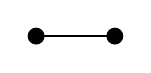
\begin{tikzpicture} 
\draw[fill=black]
(0,0) circle [radius=.1] 
(1,0) circle [radius=.1];
\draw[line width=0.3mm]
(0,0) --++ (1,0);               
\end{tikzpicture}
\caption*{$(A_2)$} \label{fig:An_cox}
\end{subfigure}
\begin{subfigure}[b]{0.1\textwidth}
\centering %=== An ===
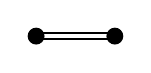
\begin{tikzpicture} 
\draw[fill=black]
(0,0) circle [radius=.1] 
(1,0) circle [radius=.1];
\draw[line width=0.3mm]
(0,+.04) --++ (1,0)
(0,-.04) --++ (1,0);              
\end{tikzpicture}
\caption*{$(B_2)$} \label{fig:An_cox}
\end{subfigure}
\begin{subfigure}[b]{0.1\textwidth}
\centering %=== An ===

\begin{tikzpicture} 
\draw[fill=black]
(0,0) circle [radius=.1] 
(1,0) circle [radius=.1];
\draw[line width=0.3mm]
(0,0) --++ (1,0)
(0,+.08) --++ (1,0)
(0,-.08) --++ (1,0);              
\end{tikzpicture}
\caption*{$(G_2)$} \label{fig:An_cox}
\end{subfigure}
\end{figure}

\end{example}


\begin{proposition}
For $R$ to be irreducible, it is necessary and sufficient that its Coxeter graph should be connected and nonempty.
\end{proposition}
\begin{proof}
Assume first that $R$ is not irreducible. That is, $R$ is the sum of two nonempty subsystems $R_1$ and $R_2$. Let $S_1$ and $S_2$ be their bases respectively. Since $S_1$ and $S_2$ are orthogonal, $n(\alpha,\beta)=0$ for all $\alpha \in S_1$ and $\beta \in S_2$. Hence the Coxeter graph is nonempty, but disconnected. 

Conversely, if the Coxeter graph of $R$ is disconnected, then there exists a separation $S=S_1\cup S_2$ of the base $S$ into nonempty subsets $S_1$ and $S_2$ such that no root in $S_1$ is connected to a root in $S_2$. Hence $n(\alpha,\beta)=0$ for all $\alpha \in S_1$ and $\beta \in S_2$. Thus $S_1$ and $S_2$ are orthogonal meaning that if $V_1$ and $V_2$ are the vector spaces spanned by $S_1$ and $S_2$ respectively, then $s_\alpha(S) = s_\alpha(S_1) \cup s_\alpha (S_2) \subseteq V_1 \cup V_2$ for all $\alpha \in S$. Hence $R$ is contained in $V_1 \cup V_2$ meaning that $R$ is not irreducible.
\end{proof}

\begin{definition}[Admissable]
A nonempty set $A=\{v_1,v_2,...,v_n\}$ of linearly independent vectors in a real inner product space is said to be \textit{admissable} if
\begin{itemize}
\item[a)] $(v_i,v_i)=1$ for all $i$ and $(v_i,v_j)\leq 0$ whenever $i\neq j$.
\item[b)] $4(v_i,v_j)^2\in \{0,1,2,3\}$ for all $i\neq j$.
\end{itemize}
The Coxeter graph consisting of $n$ vertices where the vertices $v_i$ and $v_j$ are connected by $N_{ij}=4(v_i,v_j)^2$ edges is referred to as an \textit{admissable graph} if it is connected.
\end{definition}

\noindent
Recalling $N_{ij}=n(\alpha_i,\alpha_j)n(\alpha_j,\alpha_i)=4\cos^2 \theta$ it is clear that the Coxeter graph is independent of the length of the roots. Hence it is convenient to introduce the set
\[
A=\left\{\frac{\alpha}{|\alpha|}\big| \alpha \in S \right\}
\]
which is admissable by lemma \ref*{lem:leq0} and the observation that $N_{ij}=4(\alpha_i,\alpha_j)^2\in\{0,1,2,3\}$ for distinct $\alpha_i,\alpha_j \in A$. That is, every reduced root system gives rise to an admissable set. If the root system is irreducible, then it will have a Coxeter graph which is admissable.

It should here be noted that any subset of an admissable set is itself admissable. 


\begin{lemma} \label{lemma:VertexMoreThanEdge}
In an admissable graph the number of pairs of vertices joined by at least one edge is at most one less than the number vertices.
\end{lemma}
\begin{proof}
Let $A=\{\alpha_1,...,\alpha_n\}$ be admissable and set $\alpha = \sum_{i=1}^n \alpha_i$. Since $A$ is linearly independent $\alpha \neq 0$ and thus 
\[
(\alpha,\alpha) = \sum_{i=1}^n \sum_{j=1}^n (\alpha_i,\alpha_j) = n + \sum_{j>i} 2(\alpha_i,\alpha_j) > 0.
\]
Using that $\sqrt{N_{ij}}=-2(\alpha_i,\alpha_j)$ for all $\alpha_i,\alpha_j\in A$ it follows that
\[
n > \sum_{j>i} -2(\alpha_i,\alpha_j) = \sum_{j>i} \sqrt{ N_{ij} } \geq N
\]
where $N$ is the number of nonzero $N_{ij}$ with $i\neq j$. Hence $n>N$, which is the wanted result.
\end{proof}

\begin{corollary}
An admissable graph cannot contain any cycles. 
\end{corollary}
\begin{proof}
Assume $A$ is an admissable set whose admissable graph contains a cycle. Then the subset $A'$ of $A$ containing this cycle is admissable. The graph is $A'$ does then have the same number of pairs of connected vertices as it has vertices. This contradicts the previous lemma.
\end{proof}



\begin{lemma} \label{lemma:NoMoreThanThree}
No vertex in the Coxeter graph can be incident to four of more egdes. 
\end{lemma}
\begin{proof}
Let $\alpha_1,...,\alpha_n$ be all the vertices in an admissable graph joined to $\alpha$. Since the graph cannot contain any cycles we must have $N_{ij}=0$ for all $i\neq j$. That is, for all $i\neq j$ the vectors $\alpha_i$ and $\alpha_j$ are orthogonal. The basis $\alpha_1,...,\alpha_n,\alpha$ may be orthonormalized using the Gram-Shmidt process adding the vector $\alpha_0$ which is proportional to $\alpha$. This gives an orthonormal basis $\alpha_0,\alpha_1,...,\alpha_n$ allowing us to write $\alpha = \sum_{i=0}^n (\alpha,\alpha_i)\alpha_i$. Since $|\alpha|=1$ we must have $(\alpha,\alpha) = \sum_{i=0}^n (\alpha,\alpha_i)^2 = 1$ and since $(\alpha,\alpha_0)^2>0$ it follows that $\sum_{i=1}^n (\alpha,\alpha_i)^2 < 1$.
Since $\alpha$ is joined to all $\alpha_i$ we have $(\alpha,\alpha_i)^2 \geq \frac{1}{4}$ and thus $\frac{1}{4}n \leq \sum_{i=1}^n (\alpha,\alpha_i)^2 < 1$, so $n<4$.
\end{proof}

\noindent
It follows that the only admissable graph with a triple edge is
\begin{figure}[H]
\centering

\begin{tikzpicture}
\draw[fill=black]
(0,0) circle [radius=.1] 
(1,0) circle [radius=.1];
\draw[line width=0.3mm]
(0,0) --++ (1,0)
(0,+.08) --++ (1,0)
(0,-.08) --++ (1,0);
\end{tikzpicture}
\end{figure}

\begin{definition}[branch]
If a vertex in a graph is part of more than two pairs of vertices that are connected by an edge, then the vertex is said to be a \textit{branch} in the graph.
\end{definition}


\begin{lemma} \label{lemma:ShrinkingLemma}
If an admissable graph has a subgraph $\{v_1,...,v_k\}$ which is a line, then the graph where the whole line has been collapsed to a single vertex $v=\sum_{i=1}^k v_i$ is admissable. Moreover, if $w=\sum_{i=1}^k i v_i$ then $(w,w)=\frac{1}{2}k(k+1)$.
\end{lemma}
\begin{proof}
Let $A$ be the admissable set consisting of the original graph where the line $\{v_1,...,v_k\}$ has been collapsed to the element $v$. Since $A'$ clearly is linearly independent it suffices to show that $(v,v)=1$, $(v,\alpha)\leq 0$ and $4(v,\alpha)^2\in \{0,1,2,3\}$ for all $\alpha\in A'-\{v\}$. First note that since the original set is admissable $(v,\alpha)=\sum_{i=1}^k (v_i,\alpha) \leq 0$. Further, since $\{v_1,...,v_k\}$ is a line we must have $2(v_i,v_{i+1})=-1$ and thus also
\[
(v,v)
= \sum_{i=1}^k \sum_{j=1}^k (v_i,v_j)
= k + \sum_{i=1}^{k-1} 2(v_i,v_{i+1})
= k-(k-1)
= 1.
\]
Now choose $\alpha\in A'-\{v\}$ and see that since the original graph is admissable, and thus does not contain any cycles, there is at most one $v_i$ so that $(v_i,\alpha)\neq 0$. Hence $(v,\alpha)=(v_i,\alpha)$ and thus also $4(v,\alpha)^2=4(v_i,\alpha)^2 \in \{0,1,2,3\}$.

To prove the last part observe that $(v_i,v_i)=1$ and $2(v_i,v_{i+1})=-1$ for all $1\leq i < k$ with $(v_i,v_j)=0$ if neither $i=j$ nor $j=i+1$. We then find that
\[
(w,w) 
= \sum_{i=1}^k i^2 + \sum_{i=1}^{k-1} 2i(i+1)(v_i,v_{i+1})
= k^2 - \sum_{i=1}^{k-1} i
= \frac{1}{2}k(k+1).
\]
\end{proof}

\begin{corollary}
Let $\Gamma$ be an admissable graph, then:
\begin{itemize}
\item[a)] $\Gamma$ has no more than one double edge. 
\item[b)] $\Gamma$ has no more than one branch.
\item[c)] $\Gamma$ does not have both a branch and a double edge. 
\end{itemize}
\end{corollary}
\begin{proof}
To prove $a)$ assume an admissable graph contains two double edges. Being connected, it must contain a subgraph of the form 
\begin{center}
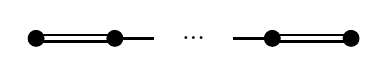
\begin{tikzpicture} 
\draw[fill=black]
(0,0) circle [radius=.1] 
(1,0) circle [radius=.1] 
(3,0) circle [radius=.1] 
(4,0) circle [radius=.1];
\draw[line width=0.3mm] 
(0,+.04) --++ (1,0) 
(0,-.04) --++ (1,0) 
(1,0) --++ (0.5,0)  
(3,0) --++ (-0.5,0) 
(3,+.04) --++ (1,0) 
(3,-.04) --++ (1,0);
\draw (2,0) node {$...$};                    
\end{tikzpicture}
\end{center}
By lemma \ref*{lemma:ShrinkingLemma}, the graph
\begin{center}
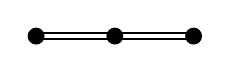
\begin{tikzpicture} 
\draw[fill=black](0,0) circle [radius=.1] (1,0) circle [radius=.1](2,0) circle [radius=.1];
\draw[line width=0.3mm](0,+.04) --++ (1,0)(0,-.04) --++ (1,0)(1,+.04) --++ (1,0)
(1,-.04) --++ (1,0);         
\end{tikzpicture}
\end{center}
should also be admissable. This contradicts lemma \ref*{lemma:NoMoreThanThree}. Since the same argument holds if one, or both, of the double edges are replaced by a branch $b)$ and $c)$ follows.
\end{proof}

\begin{proposition} \label{lemma:HavingOneDoubleEdge}
If an admissable graph has a double edge, then it is of the form
\begin{center}
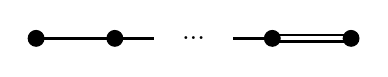
\begin{tikzpicture}
\draw[fill=black]
(0,0) circle [radius=.1] 
(1,0) circle [radius=.1]
(3,0) circle [radius=.1]
(4,0) circle [radius=.1];
\draw[line width=0.3mm]
(0,0) --++ (1,0)
(1,0) --++ (0.5,0) 
(3,0) --++ (-0.5,0)
(3,+.04) --++ (1,0)
(3,-.04) --++ (1,0);  
\draw (2,0) node {$...$};  
\end{tikzpicture}
 \ \ or \ \
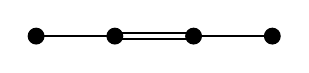
\begin{tikzpicture}
\draw[fill=black]
(0,0) circle [radius=.1] 
(1,0) circle [radius=.1]
(2,0) circle [radius=.1]
(3,0) circle [radius=.1];
\draw[line width=0.3mm]
(0,0) --++ (1,0)
(1,+.04) --++ (1,0) 
(1,-.04) --++ (1,0)
(2,0) --++ (1,0); 
\end{tikzpicture}
.
\end{center}
\end{proposition}
\begin{proof}
From the corollary to lemma \ref*{lemma:ShrinkingLemma} it follows that the graph must be of the form 
\begin{center}
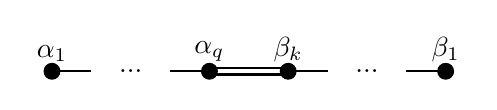
\begin{tikzpicture}
\draw[fill=black]
(0,0) circle [radius=.1] node[above]{$\alpha_1$}
(2,0) circle [radius=.1] node[above]{$\alpha_q$}
(3,0) circle [radius=.1] node[above]{$\beta_k$}
(5,0) circle [radius=.1] node[above]{$\beta_1$};
\draw[line width=0.3mm]
(0,0) --++ (0.5,0) 
(2,0) --++ (-0.5,0)
(3,0) --++ (0.5,0) 
(5,0) --++ (-0.5,0)
(2,+.04) --++ (1,0)
(2,-.04) --++ (1,0);  
\draw (1,0) node {$...$};  
\draw (4,0) node {$...$};  
\end{tikzpicture}
\end{center}
where we without loss of generality can assume that $s\geq k$. From lemma \ref*{lemma:ShrinkingLemma} it follows that if $\alpha = \sum_{i=1}^q i\alpha_i$ and $\beta = \sum_{i=1}^k i \beta_i$ then 
\[
(\alpha,\alpha)=\frac{1}{2}q(q+1) \mbox{ and } (\beta, \beta) = \frac{1}{2}k(k+1).
\]
Since $4(\alpha_i,\beta_j)^2=2$ for $i=q$ and $j=k$ and zero otherwise, it follows that $(\alpha,\beta)^2=(q\alpha_q,k\beta_k)^2=\frac{1}{2}q^2k^2$. Invoking the Cauchy-Schwartz inequality we find that $(\alpha,\beta)^2 < (\alpha,\alpha)(\beta,\beta)$ since $\alpha$ and $\beta$ are not proportional. After cancelling this gives $2qk<(q+1)(k+1)$ which may we simplified into $qk<q+k+1$. This is only satisfied for $k=1$ or $q=k=2$, which is the desired result.
\end{proof}


\begin{theorem} \label{theorem:CoxeterOfAdmissable}
Any admissable graph is of the form
\begin{figure}[H]
%\begin{center}
\begin{subfigure}[b]{0.5\textwidth}
\centering %=== An ===
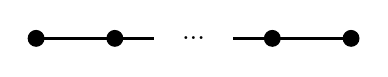
\begin{tikzpicture} 
\draw[fill=black]
(0,0) circle [radius=.1] 
(1,0) circle [radius=.1]
(3,0) circle [radius=.1]
(4,0) circle [radius=.1];
\draw[line width=0.3mm]
(0,0) --++ (1,0)
(1,0) --++ (0.5,0) 
(3,0) --++ (-0.5,0)
(3,0) --++ (1,0);  
\draw (2,0) node {$...$};                    
\end{tikzpicture}
\caption*{$(A_n)$} \label{fig:An_cox}
\end{subfigure}
\begin{subfigure}[b]{0.5\textwidth} 
\centering
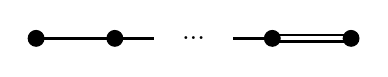
\begin{tikzpicture}
\draw[fill=black]
(0,0) circle [radius=.1] 
(1,0) circle [radius=.1]
(3,0) circle [radius=.1]
(4,0) circle [radius=.1];
\draw[line width=0.3mm]
(0,0) --++ (1,0)
(1,0) --++ (0.5,0) 
(3,0) --++ (-0.5,0)
(3,+.04) --++ (1,0)
(3,-.04) --++ (1,0);  
\draw (2,0) node {$...$};  
\end{tikzpicture}
\caption*{$(B_n)$} \label{fig:Bn_cox}
\end{subfigure}
\begin{subfigure}[b]{0.5\textwidth} 
\centering
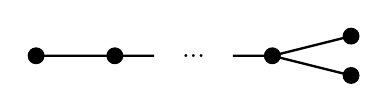
\begin{tikzpicture}
\draw[fill=black]
(0,0) circle [radius=.1] 
(1,0) circle [radius=.1]
(3,0) circle [radius=.1]
(4,+.25) circle [radius=.1]
(4,-.25) circle [radius=.1];
\draw[line width=0.3mm]
(0,0) --++ (1,0)
(1,0) --++ (0.5,0) 
(3,0) --++ (-0.5,0)
(3,0) --++ (1,+.25)
(3,0) --++ (1,-.25);
\draw (2,0) node {$...$};  
\end{tikzpicture}
\caption*{$(D_n)$} \label{fig:Dn_cox}
\end{subfigure}
\begin{subfigure}[b]{0.5\textwidth} 
\centering

\begin{tikzpicture}
\draw[fill=black]
(0,0) circle [radius=.1] 
(1,0) circle [radius=.1];
\draw[line width=0.3mm]
(0,0) --++ (1,0)
(0,+.08) --++ (1,0)
(0,-.08) --++ (1,0);
\end{tikzpicture}
\caption*{$(G_2)$} \label{fig:G2_cox}
\end{subfigure}
\begin{subfigure}[b]{0.5\textwidth} % B2 =============================================================================
\centering
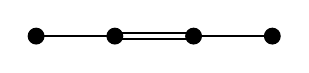
\begin{tikzpicture}
\draw[fill=black]
(0,0) circle [radius=.1] 
(1,0) circle [radius=.1]
(2,0) circle [radius=.1]
(3,0) circle [radius=.1];
\draw[line width=0.3mm]
(0,0) --++ (1,0)
(1,+.04) --++ (1,0) 
(1,-.04) --++ (1,0)
(2,0) --++ (1,0); 
\end{tikzpicture}
\caption*{$(F_4)$} \label{fig:F4_cox}
\end{subfigure}
\begin{subfigure}[b]{0.5\textwidth} 
\centering
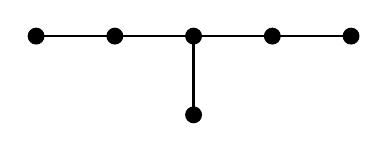
\begin{tikzpicture}
\draw[fill=black]
(0,0) circle [radius=.1] 
(1,0) circle [radius=.1]
(2,0) circle [radius=.1]
(2,-1) circle [radius=.1]
(3,0) circle [radius=.1]
(4,0) circle [radius=.1];
\draw[line width=0.3mm]
(0,0) --++ (1,0)
(1,0) --++ (1,0)
(2,0) --++ (1,0)
(3,0) --++ (1,0)
(2,0) --++ (0,-1); 
\end{tikzpicture}
\caption*{$(E_6)$} \label{fig:E6_cox}
\end{subfigure}
\begin{subfigure}[b]{0.5\textwidth}
\centering
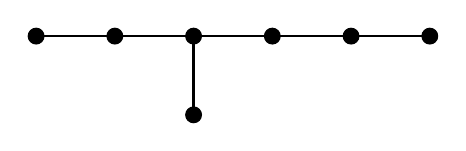
\begin{tikzpicture}
\draw[fill=black]
(0,0) circle [radius=.1] 
(1,0) circle [radius=.1]
(2,0) circle [radius=.1]
(2,-1) circle [radius=.1]
(3,0) circle [radius=.1]
(4,0) circle [radius=.1]
(5,0) circle [radius=.1];
\draw[line width=0.3mm]
(0,0) --++ (1,0)
(1,0) --++ (1,0)
(2,0) --++ (1,0)
(3,0) --++ (1,0)
(4,0) --++ (1,0)
(2,0) --++ (0,-1); 
\end{tikzpicture}
\caption*{$(E_7)$} \label{fig:E7_cox}
\end{subfigure}
\begin{subfigure}[b]{0.5\textwidth} 
\centering
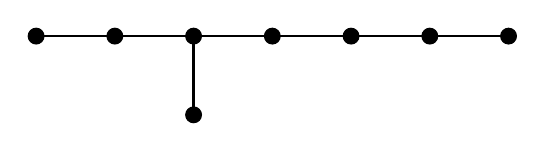
\begin{tikzpicture}
\draw[fill=black]
(0,0) circle [radius=.1] 
(1,0) circle [radius=.1]
(2,0) circle [radius=.1]
(2,-1) circle [radius=.1]
(3,0) circle [radius=.1]
(4,0) circle [radius=.1]
(5,0) circle [radius=.1]
(6,0) circle [radius=.1];
\draw[line width=0.3mm]
(0,0) --++ (1,0)
(1,0) --++ (1,0)
(2,0) --++ (1,0)
(3,0) --++ (1,0)
(4,0) --++ (1,0)
(5,0) --++ (1,0)
(2,0) --++ (0,-1); 
\end{tikzpicture}
\caption*{$(E_8)$} \label{fig:E8_cox}
\end{subfigure}
%\end{center}
%\caption{
%The possible connected, nonempty Coxeter graphs attached to a root system.
%}
%\label{fig:CoxeterGraphs}
\end{figure}
\end{theorem}
\begin{proof}
It suffices to show that if an admissable graph has one branch, then it is either $E_6$, $E_7$, $E_8$ or $D_n$ for some $n\geq 4$. As in the proof of lemma \ref*{lemma:HavingOneDoubleEdge}, any admissable graph with one branch must have the form
\begin{center}
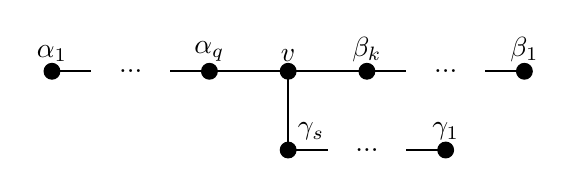
\begin{tikzpicture}
\draw[fill=black]
(0,0) circle [radius=.1] node[above]{$\alpha_1$}
(2,0) circle [radius=.1] node[above]{$\alpha_q$}
(3,0) circle [radius=.1] node[above]{$v$}
(4,0) circle [radius=.1] node[above]{$\beta_k$}
(6,0) circle [radius=.1] node[above]{$\beta_1$}
(3,-1) circle [radius=.1] node[above right]{$\gamma_s$}
(5,-1) circle [radius=.1] node[above]{$\gamma_1$};
\draw[line width=0.3mm]
(0,0) --++ (0.5,0) 
(2,0) --++ (-0.5,0)
(4,0) --++ (0.5,0) 
(6,0) --++ (-0.5,0)
(3,-1) --++ (0.5,0) 
(5,-1) --++ (-0.5,0)
(2,0) --++ (1,0)
(3,0) --++ (1,0)
(3,0) --++ (0,-1);  
\draw 
(1,0) node {$...$}
(5,0) node {$...$}
(4,-1) node {$...$};  
\end{tikzpicture}
\end{center}
where we can, without loss of generality, assume that $q\geq k \geq s$. Now, since there are no edges directly connecting the lines $\{\alpha_i\}$, $\{\beta_i\}$ and $\{\gamma_i\}$ the vectors
\[
\alpha = \sum_{i=1}^q i\alpha_i, \ \beta = \sum_{i=1}^k i\beta_i \mbox{ and } \gamma = \sum_{i=1}^s i\gamma_i
\]
are orthogonal. Define $\alpha'=\alpha/|\alpha|$, $\beta'=\beta/|\beta|$ and $\gamma'=\gamma/|\gamma|$ and see that since the set $\{ v,\alpha',\beta',\gamma'\}$ is linearly independent it is possible to construct, using the Gram-Schmidt process, a vector $v_0$ with $(v,v_0)\neq 0$ so that $\{ v_0,\alpha',\beta',\gamma'\}$ is orthonormal. We may then write $v$ as a linear combination of these vectors as
\[
v = (v,\alpha')\alpha'+(v,\beta')\beta'+(v,\gamma')\gamma'+(v,v_0)v_0
\]
and since $|v|=1$ and $(v,v_0)^2>0$ it follows that
\[
(v,\alpha')^2+(v,\beta')^2+(v,\gamma')^2< (v,\alpha')^2+(v,\beta')^2+(v,\gamma')^2+(v,v_0)^2 = |v|^2 = 1.
\]
Now observe that $(v,\alpha)^2=(v,q\alpha_q)^2=\frac{1}{4}q^2$, $(v,\beta)^2=\frac{1}{4}k^2$ and $(v,\gamma)^2=\frac{1}{4}s^2$. Invoking lemma \ref*{lemma:ShrinkingLemma} then gives 
\[
(v,\alpha')^2=\frac{2q^2}{4q(q+1)}, \ 
(v,\beta')^2=\frac{2k^2}{4k(k+1)} 
\mbox{ and }
(v,\gamma')^2=\frac{2s^2}{4s(s+1)} 
\]
which, when substituted back into the inequality, gives 
\[
\frac{q}{q+1}+\frac{k}{k+1}+\frac{s}{s+1}<2.
\]
Using that $\frac{x}{x+1}=1-\frac{1}{x+1}$ for any non-negative $x$ we may rewrite the inequality in the form
\[
\frac{1}{q+1}+\frac{1}{k+1}+\frac{1}{s+1}>1.
\]
Since $\frac{1}{2}\geq \frac{1}{s+1} \geq \frac{1}{k+1} \geq \frac{1}{q+1}$ it follows that $\frac{3}{s+1} > 1$ and thus $s=1$. Now that we know $s$ we may perform the same argument to find that $\frac{2}{k+1} > \frac{1}{2}$ giving $k\leq 2$. If $k=2$ then $q\leq 4$ and if $k=1$ then $q$ may be any positive integer.
\end{proof}





\subsection{The Dynkin diagram}
Constructing the admissable sets from a base $S$ for a reduced root system involved forcing all the elements to have the same length. Hence some information was lost. This motivates the definition of the Dynkin diagram for a reduced root system.


\begin{definition}[Dynkin diagram]
Let $R$ be a reduced root system with base $S$. The \textit{Dynkin diagram} of $R$ is the Coxeter graph of $R$ together with a symbol $>$ or $<$ on each double or triple edge. The symbol $<$ indicates that the root on the right is largest of the two, and $>$ indicates that it is the smallest. 
\end{definition}

\begin{proposition}\label{prop:DynkinEquivToCartan}
Specifying the Dynkin diagram is equivalent to specifying a Cartan matrix. 
\end{proposition}
\begin{proof}
Given any Cartan matrix $C_{ij}$, for an reduced, of dimension $n\times n$ we may always construct a Coxeter graph, and thus also a Dynkin diagram, having $n$ vertices such that every two distinct vertices $i$ and $j$ is connected by $N_{ij}=C_{ij}C_{ji}$ edges. Hence it suffices to show that a unique Cartan matrix may be constructed given a Dynkin diagram. Clearly, reordering the vertices in the Dynkin diagram could give a different Cartan matrix, but, as mentioned before, such Cartan matrices are considered equal since this only amounts to reshuffling the roots in the base. Now, consider two vertices $\alpha_i$ and $\alpha_j$ in a Dynkin diagram. If the vertices shares no edge, then $n(\alpha_i,\alpha_j)=n(\alpha_j,\alpha_i)=0$ meaning that the corresponding elements in the Cartan matrix must be $C_{ij}=C_{ji}=0$. Similarily, if the vertices are connected by a single edge then table \ref*{tab:RootsAndAngles}, together with lemma \ref*{lem:leq0}, implies that $C_{ij}=C_{ji}=-1$. If the vertices shares a double edge, then together with the edge we are provided with the information that either $|\alpha_i|>|\alpha_j|$ or $|\alpha_i|<|\alpha_j|$. In the first case lemma \ref*{lem:leq0} and table \ref*{tab:RootsAndAngles} gives $C_{ij}=-1$ and $C_{ji}=-2$, and in the second case $C_{ij}=-2$ and $C_{ji}=-1$. A similar argument shows that in the case of a triple edge, then $C_{ij}=-1$ and $C_{ji}=-3$ if $|\alpha_i|>|\alpha_j|$ and $C_{ij}=-3$ and $C_{ji}=-1$ if $|\alpha_i|<|\alpha_j|$. Repeating this for every pair of distinct vertices every non-diagonal element in the corresponding Cartan matrix is determined. Since $n(\alpha,\alpha)=2$ for all nonzero vectors the digaonal terms in the Cartan matrix are all equal to $2$. We have now specified the Cartan matrix, which is the desired result.
\end{proof}

\begin{theorem}
Any both reduced and irreducible root system $R$ is determined by one of the following Dynkin diagrams up to isomorphism:
\begin{figure}[H]
%\begin{center}
\begin{subfigure}[b]{0.5\textwidth}
\centering %=== An ===
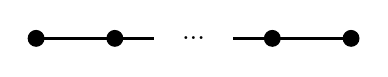
\begin{tikzpicture} 
\draw[fill=black]
(0,0) circle [radius=.1] 
(1,0) circle [radius=.1]
(3,0) circle [radius=.1]
(4,0) circle [radius=.1];
\draw[line width=0.3mm]
(0,0) --++ (1,0)
(1,0) --++ (0.5,0) 
(3,0) --++ (-0.5,0)
(3,0) --++ (1,0);  
\draw (2,0) node {$...$};                    
\end{tikzpicture}
\caption*{$(A_n)$} \label{fig:An_dyn}
\end{subfigure}
\begin{subfigure}[b]{0.5\textwidth} 
\centering
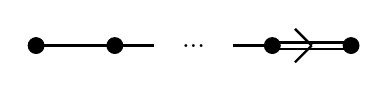
\begin{tikzpicture}
\draw[fill=black]
(0,0) circle [radius=.1] 
(1,0) circle [radius=.1]
(3,0) circle [radius=.1]
(4,0) circle [radius=.1];
\draw[line width=0.3mm]
(0,0) --++ (1,0)
(1,0) --++ (0.5,0) 
(3,0) --++ (-0.5,0)
(3,+.04) --++ (1,0)
(3,-.04) --++ (1,0);  
\draw (2,0) node {$...$}; 
% makes the arrow head
\draw[line width=0.3mm]
(3.5,0) --++ (135:.3)
(3.5,0) --++ (-135:.3); 
\end{tikzpicture}
\caption*{$(B_n)$} \label{fig:Bn_dyn}
\end{subfigure}
\begin{subfigure}[b]{0.5\textwidth} 
\centering
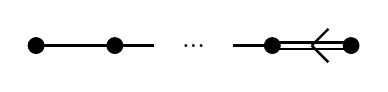
\begin{tikzpicture}
\draw[fill=black]
(0,0) circle [radius=.1] 
(1,0) circle [radius=.1]
(3,0) circle [radius=.1]
(4,0) circle [radius=.1];
\draw[line width=0.3mm]
(0,0) --++ (1,0)
(1,0) --++ (0.5,0) 
(3,0) --++ (-0.5,0)
(3,+.04) --++ (1,0)
(3,-.04) --++ (1,0);  
\draw (2,0) node {$...$};  
% makes the arrow head
\draw[line width=0.3mm]
(3.5,0) --++ (45:.3)
(3.5,0) --++ (-45:.3);
\end{tikzpicture}
\caption*{$(C_n)$} \label{fig:Cn_dyn}
\end{subfigure}
\begin{subfigure}[b]{0.5\textwidth} 
\centering
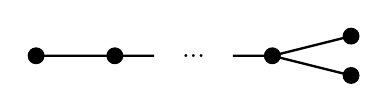
\begin{tikzpicture}
\draw[fill=black]
(0,0) circle [radius=.1] 
(1,0) circle [radius=.1]
(3,0) circle [radius=.1]
(4,+.25) circle [radius=.1]
(4,-.25) circle [radius=.1];
\draw[line width=0.3mm]
(0,0) --++ (1,0)
(1,0) --++ (0.5,0) 
(3,0) --++ (-0.5,0)
(3,0) --++ (1,+.25)
(3,0) --++ (1,-.25);
\draw (2,0) node {$...$};  
\end{tikzpicture}
\caption*{$(D_n)$} \label{fig:Dn_dyn}
\end{subfigure}
\begin{subfigure}[b]{0.5\textwidth} 
\centering
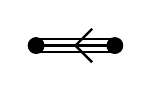
\begin{tikzpicture}
\draw[fill=black]
(0,0) circle [radius=.1] 
(1,0) circle [radius=.1];
\draw[line width=0.3mm]
(0,0) --++ (1,0)
(0,+.08) --++ (1,0)
(0,-.08) --++ (1,0);
% makes the arrow head
\draw[line width=0.3mm]
(0.5,0) --++ (45:.3)
(0.5,0) --++ (-45:.3);
\end{tikzpicture}
\caption*{$(G_2)$} \label{fig:G2_dyn}
\end{subfigure}
\begin{subfigure}[b]{0.5\textwidth} % B2 =============================================================================
\centering
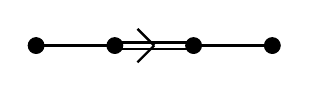
\begin{tikzpicture}
\draw[fill=black]
(0,0) circle [radius=.1] 
(1,0) circle [radius=.1]
(2,0) circle [radius=.1]
(3,0) circle [radius=.1];
\draw[line width=0.3mm]
(0,0) --++ (1,0)
(1,+.04) --++ (1,0) 
(1,-.04) --++ (1,0)
(2,0) --++ (1,0); 
% makes the arrow head
\draw[line width=0.3mm]
(1.5,0) --++ (135:.3)
(1.5,0) --++ (-135:.3);
\end{tikzpicture}
\caption*{$(F_4)$} \label{fig:F4_dyn}
\end{subfigure}
\begin{subfigure}[b]{0.5\textwidth} 
\centering
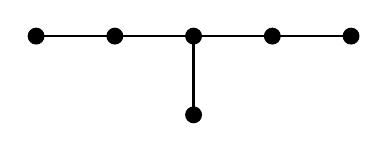
\begin{tikzpicture}
\draw[fill=black]
(0,0) circle [radius=.1] 
(1,0) circle [radius=.1]
(2,0) circle [radius=.1]
(2,-1) circle [radius=.1]
(3,0) circle [radius=.1]
(4,0) circle [radius=.1];
\draw[line width=0.3mm]
(0,0) --++ (1,0)
(1,0) --++ (1,0)
(2,0) --++ (1,0)
(3,0) --++ (1,0)
(2,0) --++ (0,-1); 
\end{tikzpicture}
\caption*{$(E_6)$} \label{fig:E6_dyn}
\end{subfigure}
\begin{subfigure}[b]{0.5\textwidth}
\centering
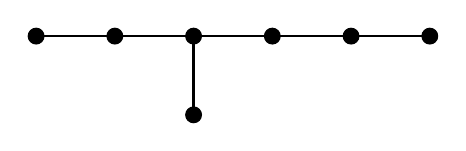
\begin{tikzpicture}
\draw[fill=black]
(0,0) circle [radius=.1] 
(1,0) circle [radius=.1]
(2,0) circle [radius=.1]
(2,-1) circle [radius=.1]
(3,0) circle [radius=.1]
(4,0) circle [radius=.1]
(5,0) circle [radius=.1];
\draw[line width=0.3mm]
(0,0) --++ (1,0)
(1,0) --++ (1,0)
(2,0) --++ (1,0)
(3,0) --++ (1,0)
(4,0) --++ (1,0)
(2,0) --++ (0,-1); 
\end{tikzpicture}
\caption*{$(E_7)$} \label{fig:E7_dyn}
\end{subfigure}
\begin{subfigure}[b]{0.5\textwidth} 
\centering
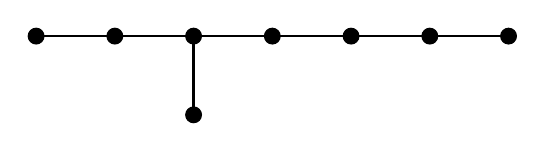
\begin{tikzpicture}
\draw[fill=black]
(0,0) circle [radius=.1] 
(1,0) circle [radius=.1]
(2,0) circle [radius=.1]
(2,-1) circle [radius=.1]
(3,0) circle [radius=.1]
(4,0) circle [radius=.1]
(5,0) circle [radius=.1]
(6,0) circle [radius=.1];
\draw[line width=0.3mm]
(0,0) --++ (1,0)
(1,0) --++ (1,0)
(2,0) --++ (1,0)
(3,0) --++ (1,0)
(4,0) --++ (1,0)
(5,0) --++ (1,0)
(2,0) --++ (0,-1); 
\end{tikzpicture}
\caption*{$(E_8)$} \label{fig:E8_dyn}
\end{subfigure}
\end{figure}
\end{theorem}
\begin{proof}
By virtue of proposition \ref*{prop:DynkinEquivToCartan} it suffices to show that if $R$ is a reduced and irreducible root system, then its Dynkin graph must be one of the diagrams above. Let $S$ be a base for $R$ and see that since the Coxeter graph of $S$ is admissable, it must, according to theorem \ref*{theorem:CoxeterOfAdmissable}, be isomorphic to one of the graphs $A_n$, $B_n$, $D_n$, $G_2$, $F_4$, $E_6$, $E_7$ or $E_8$. Now, we need only consider the Coxeter graphs containing a double or triple edge. Both in $G_2$ and in $F_4$ the added symbol $<$ or $>$ clearly result in the same Dynkin diagram, meaning that it suffices to consider the Coxeter graph $B_n$. Depending on the added symbol the Coxeter graph $B_n$ can give two different Dynkin diagrams. These are exactly the ones named $B_n$ and $C_n$.
\end{proof}



\section{The factorization of semisimple Lie algebras}
We will in this section briefly list the definitions and results, without proof, needed to understand the connection between Lie algebras and root systems. The details and proofs can be found in Serre, J.P.\cite{Serre}. 

\begin{definition}[Lie algebra]
A lie algebra $\mathfrak{g}$ is a vector space equipped with a bilinear binary operation $[\cdot,\cdot]:\mathfrak{g}\times \mathfrak{g} \rightarrow \mathfrak{g}$, called the \textit{lie bracket}, satisfying
\begin{itemize}
\item[i)](Alternativity) $[x,x]=0 \mbox{ for all } x \in \mathfrak{g}$.
\item[ii)](Jacobi identity) $[x,[y,z]]+[y,[z,x]]+[z,[x,y]]=0 \mbox{ for all } x,y,z \in \mathfrak{g}$.
\end{itemize}
\end{definition}

\noindent 
Bilinearity may be used together with alternativity to show that the lie bracket satisfies anticommutativity $[x,y]=-[y,x] \mbox{ for all } x,y \in \mathfrak{g}$.

\begin{definition}[Subalgebra and ideal]
A subspace $\mathfrak{s}$ of a lie algebra $\mathfrak{g}$ is said to be a \textit{Lie subalgebra} if $[x,y]\in \mathfrak{s}$ for all $x,y \in \mathfrak{s}$. If this holds for all $y \in \mathfrak{s}$ and $x\in \mathfrak{g}$ the subalgebra is said to be an \textit{ideal} of $\mathfrak{g}$.
\end{definition}

\noindent
For any Lie algebra, there is a canonical representation $\mbox{ad}: \mathfrak{g} \rightarrow \mbox{End}(\mathfrak{g})$ given by $x \mapsto \mbox{ad}_x$ referred to as the \textit{ajoint representation}. Here we let $[\mbox{ad}_x, \mbox{ad}_y ] = \mbox{ad}_x \circ \mbox{ad}_y - \mbox{ad}_y \circ \mbox{ad}_x$, which can be shown to satisfy alternativity and the Jacobi identity. The elements $\mbox{ad}_x(y)=[x,y]$ is referred to as the \textit{adjoint action}. 

\begin{definition}[Killing form]
The \textit{killing form} associated with a Lie algebra is a symmetric bilinear form given by $B(x,y)=\mbox{Tr}(\mbox{ad}_x \circ \mbox{ad}_y )$.
\end{definition}
\noindent
%It can be shown that the killing form is \textit{invariant}, meaning that $B\left(\left[x,y\right],z\right)+B\left(y,\left[x,z\right]\right)=0$ for all %$x,y,z \in \mathfrak{g}$.
\noindent
If we define the \textit{orthogonal space} of a subspace $\mathfrak{a}$ relative to a bilinear form $B(\cdot,\cdot)$ by $\mathfrak{a}^\bot = \left\{ x \in \mathfrak{g} \big| B(x,y)=0 \mbox{ for all } y\in \mathfrak{a} \right\}$, we say that the bilinear form is \textit{non-degenerate} on a Lie algebra $\mathfrak{g}$ if $\mathfrak{g}^\bot=0$. Using this vocabulary, we may define what is meant by a semisimple Lie algebra\footnote{One often defines a semisimple Lie algebra to be a Lie algebra with its \textit{radical}, the maximal solvable ideal, equal to zero. This definition is then a result known as the \textit{Cartan-Killing criterion}.}

\begin{definition}[Semisimple Lie algebra]
A Lie algebra $\mathfrak{g}$ is said to be \textit{semisimple} if its killing form is non-degenerate.
\end{definition}

\noindent
In the semisimple case, a \textit{Cartan subalgebra} $\mathfrak{h}$ of $\mathfrak{g}$ is the maximal abelian subalgebra. 

Now, we say that a Lie algebra is \textit{complex} if its vector field has the the complex numbers $\mathbb{C}$ as an underlying field. It turns out that in a complex semisimple Lie algebra $\mathfrak{g}$ with Cartan subalgebra $\mathfrak{h}$, every $\mbox{ad}_x$ for $x\in \mathfrak{h}$ is diagonalizable. 

\begin{definition}[Eigen-subalgebra]
Let $\mathfrak{g}$ be a complex semisimple Lie algebra and $\mathfrak{h}$ a Cartan subalgebra for $\mathfrak{g}$. For $\alpha \in \mathfrak{h}^*$ define the \textit{eigen-subalgebra}
\[
\mathfrak{g}^\alpha = \left\{ x \in \mathfrak{g} \big| [y,x]=\alpha(y)x \mbox{ for all } y \in \mathfrak{h} \right\}.
\]
The vector $\alpha$ is said to be a \textit{root} in $\mathfrak{g}$ if $\alpha \neq 0$ and $\mathfrak{g}^\alpha \neq 0$. 
\end{definition}

\begin{theorem}
Let $\mathfrak{g}$ be a complex semisimple Lie algebra and $\mathfrak{h}$ a Cartan subalgebra. If $R$ is the set of all roots of $\mathfrak{g}$, then 
\[
\mathfrak{g} = \mathfrak{h} \oplus \bigoplus_{\alpha \in R} \mathfrak{g}^\alpha.
\]
\end{theorem}


\begin{theorem}
The set $R$ of all roots in a complex, Semisimple Lie algebra $\mathfrak{g}$ is a root system in $\mathfrak{h}^*$.
\end{theorem}

\noindent
It thus turns out that classifying the indexing set $R$, gives a classification of the complex semisimple Lie algebras. Here, the special linear Lie algebra $\mathfrak{sl}_{n+1}$ corresponds to the Dynkin diagram $A_n$, while $\mathfrak{so}_{2n+1}$ and $\mathfrak{so}_{2n}$ corresponds to $B_n$ and $D_n$ respectively. The symplectic Lie algebra $\mathfrak{sp}_{2n}$ corresponds to $C_n$.





\begin{thebibliography}{99} % Bibliography - this is intentionally simple in this template

\bibitem{Serre}
 Serre, J.P., 2000. 
 \newblock \textit{Complex semisimple Lie algebras.}
 \newblock Springer Science \& Business Media.
 
\bibitem{LieAlgebrasIntroduction}
 Erdmann, K. and Wildon, M.J., 2006. 
 \newblock \textit{Introduction to Lie algebras.} 
 \newblock Springer Science \& Business Media.
 
\bibitem{SemiSimpleLieAndRepresentations}
 Cahn, R.N., 2014. 
 \newblock \textit{Semi-simple Lie algebras and their representations.}
 \newblock Courier Corporation.

\end{thebibliography}

\end{document}
